\begin{questions}

\question Responda en forma sintética sobre los siguientes conceptos: \label{ejer_1}
\begin{parts}
	\part Programa y Proceso.
	\part Defina Tiempo de retorno (\textbf{TR}) y Tiempo de espera (\textbf{TE}) para un Job.
	\part Defina Tiempo Promedio de Retorno (\textbf{TPR}) y Tiempo promedio de espera (\textbf{TPE}) para un lote de JOBS.
	\part ¿Qué es el Quantum?
	\part ¿Qué significa que un algoritmo de scheduling sea apropiativo o no apropiativo (Preemptive o Non-Preemptive)?
	\part ¿Qué tareas realizan?: \label{tipo_sched}
	\begin{subparts}		
		\subpart \textit{Short Term Scheduler}
		\subpart \textit{Long Term Scheduler}
		\subpart \textit{Medium Term Scheduler}
	\end{subparts}
	\part ¿Qué tareas realiza el \textit{Dispatcher}?
\end{parts}

\question Procesos:
\begin{parts}
	\part ¿Cuál es la información mínima que el SO debe tener sobre un proceso?¿En que estructura de datos asociada almacena dicha información?
	\part ¿Qué significa que un proceso sea “CPU Bound” y “I/O Bound”?
	\part ¿Cuáles son los estados posibles por los que puede atravesar un proceso?
	\part Explique mediante un diagrama las posibles transiciones entre los estados.
	\part ¿Que scheduler de los mencionados en \ref{ejer_1} \ref{tipo_sched} se encarga de las transiciones?
\end{parts}

\question Para los siguientes algoritmos de scheduling:
\begin{itemize}
	\item \textit{FCFS} (Fisrt Coome First Served)
	\item \textit{SJF} (Shortest Job First)
	\item \textit{Round Robin}
	\item \textit{Prioridades}
\end{itemize}
\begin{parts}
	\part Explique su funcionamiento mediante un ejemplo.
	\part ¿Alguno de ellos requiere algún parámetro para su funcionamiento?
	\part Cual es el mas adecuado según los tipos de procesos y/o SO.
	\part Cite ventajas y desventajas de su uso.
\end{parts}

\question Para el algoritmo Round Robin, existen 2 variantes:
\begin{itemize}
	\item \textbf{Timer Fijo}
	\item \textbf{Timer Variable}
\end{itemize}
\begin{parts}
	\part ¿Qué significan estas 2 variantes?
	\part Explique mediante un ejemplo sus diferencias.
	\part En cada variante ¿Dónde debería residir la información del Quantum?
\end{parts}

\question Se tiene el siguiente lote de procesos que arriban al sistema en el instante 0 (cero):
\begin{table}[h]
  \centering
  \resizebox{12pc}{!}{
  \begin{tabular}{| c | c |}
      \hline
      \bf Job & \bf Unidades de CPU \\
      \hline
      1 & 7 \\
      \hline
      2 & 15 \\
      \hline
      3 & 12 \\
      \hline
      4 & 4 \\
      \hline
      5 & 9 \\
      \hline
  \end{tabular}
  }
\end{table}
\begin{parts}
	\part Realice los diagramas de Gantt según los siguientes algoritmos de scheduling:
	\begin{subparts}
		\subpart FCFS (First Come, First Served)
		\subpart SJF (Shortest Job First)
		\subpart Round Robin con quantum = 4 y Timer Fijo
		\subpart Round Robin con quantum = 4 y Timer Variable
	\end{subparts}
	\part Para cada algoritmo calcule el TR y TE para cada job así como el TPR y el TPE.
	\part En base a los tiempos calculados compare los diferentes algoritmos.
\end{parts}

\question Se tiene el siguiente lote de procesos: \label{ejer_sched_2}
\begin{table}[h]
  \centering
  \resizebox{14pc}{!}{
  \begin{tabular}{| c | c | c |}
      \hline
      \bf Job & \bf Llegada & \bf Unidades de CPU \\
      \hline
      1 & 0 & 4 \\
      \hline
      2 & 2 & 6 \\
      \hline
      3 & 3 & 4 \\
      \hline
      4 & 6 & 5 \\
      \hline
      5 & 8 & 2 \\
      \hline
  \end{tabular}
  }
\end{table}
\begin{parts}
	\part Realice los diagramas de Gantt según los siguientes algoritmos de scheduling:
	\begin{subparts}
		\subpart FCFS (First Come, First Served)
		\subpart SJF (Shortest Job First)
		\subpart Round Robin con quantum = 1 y Timer Variable
		\subpart Round Robin con quantum = 6 y Timer Variable
	\end{subparts}
	\part Para cada algoritmo calcule el TR y TE para cada job así como el TPR y el TPE.
	\part En base a los tiempos calculados compare los diferentes algoritmos.
	\part En el algoritmo Round Robin, que conclusión se puede sacar con respecto al valor del quantum.
	\part ¿Para el algoritmo Round Robin, en que casos utilizaría un valor de quantum alto y que ventajas y desventajas obtendría?
\end{parts}

\question Una variante al algoritmo SJF es el algoritmo SJF apropiativo o SRTF (Shortest
Remaining Time First):
\begin{parts}
	\part Realice el diagrama del Gantt para este algoritmo según el lote de trabajos del ejercicio \ref{ejer_sched_2}.
	\part ¿Nota alguna ventaja frente a otros algoritmos?
\end{parts}

\question Suponga que se agregan las siguientes prioridades al lote de procesos del ejercicio \ref{ejer_sched_2}, donde un menor número indica mayor prioridad:
\begin{table}[h]
  \centering
  \resizebox{10pc}{!}{
  \begin{tabular}{| c | c |}
      \hline
      \bf Job & \bf Prioridad \\
      \hline
      1 & 3 \\
      \hline
      2 & 4 \\
      \hline
      3 & 2 \\
      \hline
      4 & 1 \\
      \hline
      5 & 2 \\
      \hline
  \end{tabular}
  }
\end{table}
\begin{parts}
	\part Realice el diagrama de Gantt correspondiente al algoritmo de planificación por prioridades según las variantes:
	\begin{subparts}
		\subpart No Apropiativa
		\subpart Apropiativa	
	\end{subparts}
	\part Calcule el TR y TE para cada job así como el TPR y el TPE.
	\part ¿Nota alguna ventaja frente a otros algoritmos? Bajo que circunstancias lo utilizaría y ante que situaciones considera que la implementación de prioridades podría no ser de mayor relevancia?
\end{parts}

\question Inanición (\textit{Starvation})
\begin{parts}
	\part ¿Qué significa?
	\part ¿Cuál/es de los algoritmos vistos puede provocarla? \label{inciso_dos_inanicion}
	\part ¿Existe alguna técnica que evite la inanición para el/los algoritmos mencionados en \ref{inciso_dos_inanicion}?
\end{parts}

\question Los procesos, durante su ciclo de vida, pueden realizar operaciones de I/O como lecturas o escrituras a disco, cintas, uso de impresoras, etc.

\hspace{20pt} El SO mantiene para cada dispositivo, que se tiene en el equipo, una cola de procesos que espera por la utilización del mismo (al igual que ocurre con la Cola de Listos y la CPU, ya que la CPU es un dispositivo mas).

\hspace{20pt} Cuando un proceso en ejecución realiza una operación de I/O el mismo es expulsado de la CPU y colocado en la cola correspondiente a el dispositivo involucrado en la operación.

\hspace{20pt} El SO dispone también de un “I/O Scheduling” que administrada cada cola de dispositivo a través de algún algoritmo (FCFS, Prioridades, etc.). Si al colocarse un proceso en la cola del dispositivo, la misma se encuentra vacía el mismo será atendido de manera inmediata, caso contrario, deberá esperar a que el SO lo seleccione según el algoritmo de scheduling establecido.

\hspace{20pt} Los mecanismos de I/O utilizados hoy en día permiten que la CPU no sea utilizada durante la operación, por lo que el SO puede ejecutar otro proceso que se encuentre en espera una vez que el proceso bloqueado por la I/O se coloca en la cola correspondiente.

\hspace{20pt} Cuando el proceso finaliza la operación de I/O el mismo retorna a la cola de listos para competir nuevamente por la utilización de la CPU.

Para los siguientes algoritmos de Scheduling:
\begin{itemize}
	\item FCFS
	\item Round Robin con quantum = 2 y timer variable.
\end{itemize}

Y suponiendo que la cola de listos de todos los dispositivos se administra mediante FCFS, realice los diagramas de Gantt según las siguientes situaciones:
\begin{parts}
	\part Suponga que al lote de procesos del ejercicio \ref{ejer_sched_2} se agregan las siguientes operaciones de entrada salida:
	\begin{table}[h]
	  \centering
	  \resizebox{12pc}{!}{
	  \begin{tabular}{| c | c |}
	      \hline
	      \bf Job & \bf I/O (rec,ins,dur) \\
	      \hline
	      1 & (R1, 2, 1) \\
	      \hline
	      2 & (R2, 3, 1) (R2, 5, 2) \\
	      \hline
	      4 & (R3, 1, 2) (R3, 3, 1) \\
	      \hline
	  \end{tabular}
	  }
	\end{table}
	\part Suponga que al lote de procesos del ejercicio \ref{ejer_sched_2} se agregan las siguientes operaciones de entrada salida:
	\begin{table}[h]
	  \centering
	  \resizebox{12pc}{!}{
	  \begin{tabular}{| c | c |}
	      \hline
	      \bf Job & \bf I/O (rec,ins,dur) \\
	      \hline
	      1 & (R1, 2, 3) (R1, 3, 2) \\
	      \hline
	      2 & (R2, 3, 2) \\
		  \hline
	      3 & (R2, 2, 3) \\		      
	      \hline
	      4 & (R1, 1, 2) \\
	      \hline
	  \end{tabular}
	  }
	\end{table}		
\end{parts}

\question Algunos algoritmos pueden presentar ciertas desventajas cuando en el sistema se cuenta con procesos ligados a CPU y procesos ligados a entrada salida. Analice las mismas para los siguientes algoritmos: \label{ventajas_desventajas_proc_ligadura}
\begin{parts}
	\part Round Robin
	\part SRTF (Shortest Remaining Time First)
\end{parts}

\question Para equiparar la desventaja planteada en el ejercicio \ref{ventajas_desventajas_proc_ligadura}), se plantea la siguiente modificación al algoritmo:

\textbf{Algoritmo VRR} (Virtual Round Robin): Este algoritmo funciona igual que el Round Robin, con la diferencia que cuando un proceso regresa de una I/O se coloca en una cola auxiliar. Cuando se tiene que tomar el próximo proceso a ejecutar, los procesos que se encuentra en la cola auxiliar tienen prioridad sobre los otros. Cuando se elije un proceso de la cola auxiliar se le otorga el procesador por tantas unidades de tiempo como le falto ejecutar en su ráfaga de CPU anterior, esto es, se le otorga la CPU por un tiempo que surge entre la diferencia del quantum original y el tiempo usado en la última ráfaga de CPU.
\begin{parts}
	\part Analice el funcionamiento de este algoritmo mediante un ejemplo. Marque en cada instante en que cola se encuentran los procesos.
	\part Realice el ejercicio 10)a) nuevamente considerando este algoritmo, con un quantum de 2 unidades y Timer Variable.
\end{parts}

\question Suponga que un SO utiliza un algoritmo de VRR con Timer Variable para el planificar sus procesos. Para ello, el quantum es representado por un contador, que es decrementado en 1 unidad cada vez que ocurre una interrupción de reloj. ¿Bajo este esquema, puede suceder que el quantum de un proceso nunca llegue a 0 (cero)? Justifique su respuesta.

\question El algoritmo SJF (y SRTF) tiene como problema su implementación, dada la dificultad de conocer la duración de la próxima ráfaga de CPU. Es posible realizar una estimación de la próxima, utilizando la media de las ráfagas de CPU para cada proceso.

Así, por ejemplo, podemos tener la siguiente formula:
\begin{equation} \label{formula_1}
S_{n+1} = \frac{1}{n} T_{n} + \frac{n-1}{n} S_{n}
\end{equation}

Donde:

	\hspace{20pt} T$_{i}$ = duración de la ráfaga de CPU i-ésima del proceso.

	\hspace{20pt} S$_{i}$ = valor estimado para el i-ésimo caso

	\hspace{20pt} S$_{i}$ = valor estimado para la primer ráfaga de CPU. No es calculado.

\begin{parts}
	\part Suponga un proceso cuyas ráfagas de CPU reales tienen como duración: 6, 4, 6, 4, 13, 13, 13 Calcule que valores se obtendrían como estimación para las ráfagas de CPU del proceso si se utiliza la formula \ref{formula_1}, con un valor inicial estimado de S$_{1}$=10. \label{inciso_a_sjf_srtf_estimacion}

	La formula anterior \ref{formula_1} le da el mismo peso a todos los casos (siempre calcula la media). Es posible reescribir la formula permitiendo darle un peso mayor a los casos mas recientes y menor a casos viejos (o viceversa). Se plantea la siguiente formula:
	\begin{equation} \label{formula_2}
	S_{n+1} = \alpha T_{n} + (1 - \alpha) S_{n}
	\end{equation}

	Con 0 $\langle$ $\alpha$ $\langle$ 1.

	\part Analice para que valores de $\alpha$ se tienen en cuenta los casos mas recientes.
	\part Para la situación planteada en a) calcule que valores se obtendrían si se utiliza la formula \ref{formula_2} con $\alpha=0,2$; $\alpha=0,5$ y $\alpha=0,8$. \label{inciso_c_sjf_srtf_estimacion}
	\part Para todas las estimaciones realizadas en \ref{inciso_a_sjf_srtf_estimacion} y \ref{inciso_c_sjf_srtf_estimacion} ¿Cuál es la que mas se asemeja a las ráfagas de CPU reales del proceso?
\end{parts}

\question Colas Multinivel

\hspace{20pt} Hoy en día los algoritmos de planificación vistos se han ido combinando para formar algoritmos más eficientes. Así surge el algoritmo de Colas Multinivel, donde la cola de procesos listos es divida en varias colas, teniendo cada una su propio algoritmo de planificación.
\begin{parts}
	\part Suponga que se tienen dos tipos de procesos: \textit{Interactivos} y \textit{Batch}. Cada uno de estos procesos se coloca en una cola según su tipo. ¿Qué algoritmo de los vistos utilizaría para administrar cada una de estas colas?.

	A su vez, se utiliza un algoritmo para administrar cada cola que se crea. Así, por ejemplo, el algoritmo podría determinar mediante prioridades sobre que cola elegir un proceso. \label{inciso_a_colas_multinivel}
	\part Para el caso de las dos colas vistas en \ref{inciso_a_colas_multinivel}: ¿Qué algoritmo utilizaría para planificarlas?
\end{parts}

\question Suponga que en un SO se utiliza un algoritmo de planificación de colas multinivel. El mismo cuenta con 3 colas de procesos listos, en las que los procesos se encolan en una u otra según su prioridad. Hay 3 prioridades (1 , 2 , 3), donde un menor número indica mayor prioridad. \label{ejer_sched_cola_multi_1}
\hspace{20pt} Se utiliza el algoritmo de prioridades para la administración entre las colas.

\hspace{20pt} Se tiene el siguiente lote de procesos a ser procesados con sus respectivas operaciones de I/O:

\begin{table}[h]
  \centering
  \resizebox{15pc}{!}{
  \begin{tabular}{| c | c | c | c | c |}
      \hline
      \bf Job & \bf Llegada & \bf CPU & \bf I/O (rec,ins,dur) & \bf Prioridad \\
      \hline
      1 & 0 & 9 & (R1, 4, 2) (R2, 6, 3) (R1, 8, 3) & 1 \\
      \hline
      2 & 1 & 5 & (R3, 3, 2) (R3, 4, 2) & 2 \\
      \hline
      3 & 2 & 5 & (R1, 4, 1) & 3 \\
      \hline
      4 & 3 & 7 & (R2, 1, 2) (R2, 5, 3) & 2 \\
      \hline
      5 & 5 & 5 & (R1, 2, 3) (R3, 4, 3) & 1 \\
      \hline
  \end{tabular}
  }
\end{table}

Suponiendo que las colas de cada dispositivo se administran a trabes de FCFS y que cada cola de procesos listos se administra por medio de un algoritmo RR con un quantum de 3 unidades y Timer Variable, realice un diagrama de Gantt:
\begin{parts}
	\part Asumiendo que NO hay apropiación entre los procesos. \label{inciso_a_sched_cola_multi}
	\part Asumiendo que hay apropiación entre los procesos. \label{inciso_b_sched_cola_multi}
\end{parts}

\question En el esquema de Colas Multinivel, cuando se utiliza un algoritmo de prioridades para administrar las diferentes colas los procesos pueden sufrir starvation. \label{ejer_sched_cola_multi_2}

\hspace{20pt} La técnica de envejecimiento se puede aplicar a este esquema, haciendo que un proceso cambie de una cola de menor prioridad a una de mayor prioridad, después de cierto periodo de tiempo que el mismo se encuentra esperando en su cola. Luego de llegar a una cola en la que el proceso llega a ser atendido, el mismo retorna a su cola original.

\hspace{20pt} Por ejemplo: Un proceso con prioridad 3 esta en cola su cola correspondiente. Luego de X unidades de tiempo, el proceso se mueve a la cola de prioridad 2. Si en esta cola es atendido, retorna a su cola original, en caso contrario luego de sucederse otras X unidades de tiempo el proceso de mueve a la cola de prioridad 1. Esta última acción se repite hasta que el proceso obtiene la CPU, situación que hace que el mismo vuelva a su cola original.
\begin{parts}
	\part Para los casos \ref{inciso_a_sched_cola_multi} y \ref{inciso_b_sched_cola_multi} del ejercicio \ref{ejer_sched_cola_multi_1} realice el diagrama de Gantt considerando además que se tiene un envejecimiento de 4 unidades.
\end{parts}

\question La situación planteada en el ejercicio \ref{ejer_sched_cola_multi_2}, donde un proceso puede cambiar de una cola a otra, se la conoce como Colas Multinivel con Realimentación.

\hspace{20pt} Suponga que se quiere implementar un algoritmo de planificación que tenga en cuenta el tiempo de ejecución consumido por el proceso, penalizando a los que más tiempo de ejecución tienen. (Similar a la tarea del algoritmo SJF que tiene en cuenta el
tiempo de ejecución que resta).

\hspace{20pt} Utilizando los conceptos vistos de Colas Multinivel con Realimentación indique que colas implementaría, que algoritmo usaría para cada una de ellas así como para la administración de las colas entre sí.

\hspace{20pt} Tenga en cuenta que los procesos no deben sufrir inanición.

\question Un caso real: “Unix Clasico “ (SVR3 y BSD 4.3)

\hspace{20pt} Estos sistemas estaban dirigidos principalmente a entornos interactivos de tiempo compartido. El algoritmo de planificación estaba diseñado para ofrecer buen tiempo de respuesta a usuarios interactivos y asegurar que los trabajos de menor prioridad (en segundo plano) no sufrieran inanición.

\hspace{20pt} La planificación tradicional usaba el concepto de colas multinivel con realimentación, utilizando RR para cada uno de las colas y realizando el cambio de proceso cada un segundo (quantum). La prioridad de cada proceso se calcula en función de la clase de proceso y de su historial de ejecución. Para ello se aplican las siguientes funciones:

\begin{equation} \label{formula_3}
CPU _{j}(\emph{i}) = \frac{CPU _{j}(\emph{i}-1)}{2}
\end{equation}
\begin{equation} \label{formula_4}
P_{j}(\emph{i}) = \emph{Base}_{j} + \frac{CPU _{j}(\emph{i})}{2} + \emph{nice}_{j}
\end{equation}

donde:

\hspace{20pt} \emph{CPU$_{j}$(i)} = Media de la utilización de la CPU del proceso j en el intervalo \emph{i}.

\hspace{20pt} \emph{P$_{j}$(i)} = Prioridad del proceso \emph{j} al principio del intervalo \emph{i} (los valores inferiores
indican prioridad más alta).

\hspace{20pt} \emph{Base$_{j}$} = Prioridad base del proceso \emph{j}.

\hspace{20pt} \emph{Nice$_{j}$} = Factor de ajuste.

La prioridad del proceso se calcula cada segundo y se toma una nueva decisión de planificación. El propósito de la prioridad base es dividir los procesos en bandas fijas de prioridad. Los valores de CPU y nice están restringidos para impedir que un proceso salga de la banda que tiene asignada. Las bandas definidas, en orden
decreciente de prioridad, son:
\begin{itemize}
	\item Intercambio
	\item Control de Dispositivos de I/O por bloques
	\item Gestión de archivos
	\item Control de Dispositivos de I/O de caracteres
	\item Procesos de usuarios
\end{itemize}
Veamos un ejemplo:
Supongamos 3 procesos creados en el mismo instante y con prioridad base 60 y un valor nice de 0. El reloj interrumpe al sistema 60 veces por segundo e incrementa un contador para el proceso en ejecución.

Los sectores en celeste representan el proceso en ejecución.
\begin{figure}[h]
	\centering
	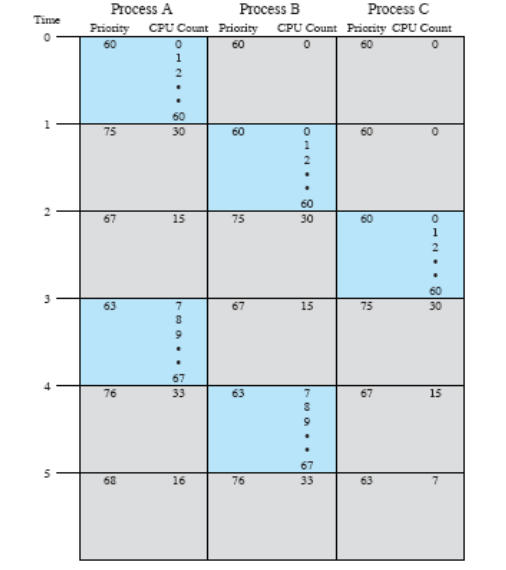
\includegraphics[scale=0.5]{images/unix_classic_real_case.png}
\end{figure}

\begin{parts}
	\part Analizando la jerarquía descripta para las bandas de prioridades: ¿Que tipo de actividad considera que tendrá más prioridad? ¿Por qué piensa que el scheduler prioriza estas actividades?
	\part Para el caso de los procesos de usuarios, y analizando las funciones antes descriptas: ¿Qué tipo de procesos se encarga de penalizar? (o equivalentemente se favorecen). Justifique
	\part La utilización de RR dentro de cada cola: ¿Verdaderamente favorece al sistema de Tiempo Compartido? Justifique.
\end{parts}

\question A cuáles de los siguientes tipos de trabajos:
\begin{parts}
	\part cortos acotados por CPU
	\part cortos acotados por E/S
	\part largos acotados por CPU
	\part largos acotados por E/S
\end{parts}
benefician las siguientes estrategias de administración:
\begin{parts}
	\part prioridad determinada estáticamente con el método del más corto primero (SJF).
	\part prioridad dinámica inversamente proporcional al tiempo transcurrido desde la última operación de E/S.
\end{parts}

\question Explicar porqué si el quantum "q" en Round-Robin se incrementa sin límite, el método se aproxima a FIFO.

\question Los sistemas multiprocesador pueden clasificarse en:
\begin{itemize}
	\item \underline{\textbf{Homogéneos}}: Los procesadores son iguales. Ningún procesador tiene ventaja física sobre el resto.
	\item \underline{\textbf{Heterogéneos}}: Cada procesador tiene su propia cola y algoritmo de planificación.
\end{itemize}
Otra clasificación posible puede ser:
\begin{itemize}
	\item \underline{\textbf{Multiprocesador débilmente acoplados}}: Cada procesador tiene su propia memoria principal y canales.
	\item \underline{\textbf{Procesadores especializados}}: Existe uno o más procesadores principales de propósito general y varios especializados controlados por el primero (ejemplo procesadores de E/S, procesadores Java, procesadores Criptográficos, etc.).
	\item \underline{\textbf{Multiprocesador fuertemente acoplado}}: Consta de un conjunto de procesadores que comparten una memoria principal y se encuentran bajo el control de un Sistema Operativo
\end{itemize}
\begin{parts}
	\part ¿Con cuál/es de estas clasificaciones asocia a las PCs de escritorio habituales?
	\part ¿Qué significa que la asignación de procesos se realice de manera simétrica?
	\part ¿Qué significa que se trabaje bajo un esquema Maestro/esclavo?
\end{parts}

\question Asumiendo el caso de procesadores homogéneos:
\begin{parts}
	\item ¿Cuál sería el método de planificación más sencillo para asignar CPUs a los procesos?
	\item Cite ventajas y desventajas del método escogido
\end{parts}

\question Indique brevemente a que hacen referencia los siguientes conceptos:
\begin{parts}
	\item Huella de un proceso en un procesador
	\item Afinidad con un procesador
	\item ¿Por qué podría ser mejor en algunos casos que un proceso se ejecute en el mismo procesador?
	\item ¿Puede el usuario en \emph{Windows} cambiar la afinidad de un proceso? ¿y en \emph{GNU/Linux}?
	\item Investigue el concepto de balanceo de carga (load balancing).
	\item Compare los conceptos de afinidad y balanceo de carga y como uno afecta al otro.
\end{parts}

\question Si a la tabla del ejercicio \ref{ejer_sched_2} la modificamos de la siguiente manera:
\begin{table}[h]
  \centering
  \resizebox{15pc}{!}{
  \begin{tabular}{| c | c | c | c |}
      \hline
      \bf Job & \bf Llegada & \bf CPU & \bf Afinidad \\
      \hline
      1 & 0 & 4 & CPU0 \\
      \hline
      2 & 2 & 6 & CPU0 \\
      \hline
      3 & 3 & 4 & CPU1 \\
      \hline
      4 & 6 & 5 & CPU1 \\
      \hline
      5 & 8 & 2 & CPU0 \\
      \hline
  \end{tabular}
  }
\end{table}
Y considerando que el scheduler de los Sistemas Operativos de la familia \emph{Windows} utiliza un mecanismo denominado preferred processor (procesador preferido). El scheduler usa el procesador preferido a modo de afinidad cuando el proceso esta en estado ready. De esta manera el sheduler asigna este procesador a la tarea si este está libre.
\begin{parts}
	\part Ejecute el esquema anterior utilizando el algoritmo anterior.
	\part Ejecute el esquema anterior. Pero ahora si el procesador preferido no está libre es asignado a otro procesador. Luego el procesador preferido de cada job es el último en el cual ejecuto.
	\part Para cada uno de los casos calcule el tiempo promedio de retorno y el tiempo promedio de espera.
	\part ¿Cuál de las dos alternativas planteadas es mas performante?
\end{parts}

\end{questions}